%%%%%%%%%%%%%%%%%%%%%%%%%%% asme2ej.tex %%%%%%%%%%%%%%%%%%%%%%%%%%%%%%%
% Template for producing ASME-format journal articles using LaTeX    %
% Written by   Harry H. Cheng, Professor and Director                %
%              Integration Engineering Laboratory                    %
%              Department of Mechanical and Aeronautical Engineering %
%              University of California                              %
%              Davis, CA 95616                                       %
%              Tel: (530) 752-5020 (office)                          %
%                   (530) 752-1028 (lab)                             %
%              Fax: (530) 752-4158                                   %
%              Email: hhcheng@ucdavis.edu                            %
%              WWW:   http://iel.ucdavis.edu/people/cheng.html       %
%              May 7, 1994                                           %
% Modified: February 16, 2001 by Harry H. Cheng                      %
% Modified: January  01, 2003 by Geoffrey R. Shiflett                %
% Use at your own risk, send complaints to /dev/null                 %
%%%%%%%%%%%%%%%%%%%%%%%%%%%%%%%%%%%%%%%%%%%%%%%%%%%%%%%%%%%%%%%%%%%%%%

%%% use twocolumn and 10pt options with the asme2ej format
%% \documentclass[twocolumn,10pt]{asme2ej}
\documentclass[]{asme2ej}

\usepackage{amsmath}
\usepackage{graphicx} %% for loading jpg figures
\usepackage{hyperref}   % to set up hyperlinks
\hypersetup{
	colorlinks=true,
	linkcolor=blue,
	citecolor=blue,
	urlcolor=blue,
}
\usepackage[square,numbers]{natbib}


\newtheorem{conjecture}{Conjecture}
\newtheorem{corollary}{Corollary}
\newtheorem{theorem}{Theorem}

%% The class has several options
%  onecolumn/twocolumn - format for one or two columns per page
%  10pt/11pt/12pt - use 10, 11, or 12 point font
%  oneside/twoside - format for oneside/twosided printing
%  final/draft - format for final/draft copy
%  cleanfoot - take out copyright info in footer leave page number
%  cleanhead - take out the conference banner on the title page
%  titlepage/notitlepage - put in titlepage or leave out titlepage
%
%% The default is oneside, onecolumn, 10pt, final


\title{A Novel Passive Ferrofluid One-way (Check) Valve Based on Energy Minimization}

%%% first author
\author{Lisa Kotowski

}
\author{Veronica Stuckey
  \affiliation{
    Biomedical Engineer, University of Texas at Austin \\
    Email:  stuckey002@gmail.com
    }
}

%%% second author
%%% remove the following entry for single author papers
%%% add more entries for additional authors
\author{Robert L. Read
\affiliation{
  Founder, Public Invention\\
  Email: read.robert@gmail.com
    }
}

%%% third author
%%% remove the following entry for single author papers
%%% add more entries for additional authors

\begin{document}

\maketitle

%%%%%%%%%%%%%%%%%%%%%%%%%%%%%%%%%%%%%%%%%%%%%%%%%%%%%%%%%%%%%%%%%%%%%%
\begin{abstract}

Small pumps and valves enable flow management in microfluidic systems.
A novel passive ferrofluid check valve is presented.
The valve consists of only a
unique channel-and-chamber geometry, ferrofluid, and a stationary
magnetic field.
The flow is determined only by the inlet and output pressure,
and the magnetic field is completely static.
The prototype valve and experimental setup are explained
and performance of the valves cracking and collapse pressure reported.
This initial design can be used for microfluid handling and lab-on-a-chip
applications.

Additionaly we present a theory of operation based on energy minimization
and compare predicted performance to actual performance.
\end{abstract}

%%%%%%%%%%%%%%%%%%%%%%%%%%%%%%%%%%%%%%%%%%%%%%%%%%%%%%%%%%%%%%%%%%%%%%
\section{Introduction}

Ferrofluid can be manipulated by electronically controlled magnetic
fields to exert force on fluids\cite{torres2014recent,kole2021engineering,ozbey2015modeling}.
This makes it possible to build pneumatic or hydraulic
devices, perhaps on very small scales,
such as a single chip\cite{yamahata2003ferrofluid,hatch2001ferrofluidic}, to
miniaturize fluid handling.
This has been proposed for biomedical purposes\cite{michelson2019novel}
that would use water or body fluids,
although this paper reports only on experiments done with air.
Miniature pumps and valves could be used to make a “lab on a chip” (LOC) or
even to heat or cool different chip areas.

A fundamental component of such
devices is the {\em check} or one-way valve.
Two check
valves on either side of a chamber whose volume can vary creates a
positive displacement pump.
A perfect check valve opens or
{\em cracks} with minimal pressure on the inlet side and sustains maximal
pressure on the outlet side before {\em collapse},
allowing fluid to flow in only one
direction. Following\cite{hartshorne2004ferrofluid} we call the maximum pressure
differential the valve can resist in the direction it is intended to
check or block (from outlet to inlet) the {\em sustainable} or {\em collapse} pressure.

This article is a brief report on an initial but functioning design of a
passive ferrofluid check valve (PFCV) that has no moving
parts except for the ferrofluid bolus itself, which is stationary
in normal operation.
By passive, the authors
mean a check valve that functions without changes to the magnetic
field affecting the bolus, whether that field is induced by a
permanent magnet or an electromagnet.
That is, the flow is determined
purely by the difference between the inlet port pressure and the
outlet port pressure.
To our knowledge, no passive
ferrofluid check valve has been previously reported, despite being an
active area of research and despite such a valve having
significant advantages for operation and especially
fabrication over valves with moving parts.

%%%%%%%%%%%%%%%%%%%%%%%%%%%%%%%%%%%%%%%%%%%%%%%%%%%%%%%%%%%%%%%%%%%%%%
\section{Related Research}

A number of papers report on ferrofluid pumps, focusing in particular
on micropump and lab-on-a-chip applications\cite{ozbey2015modeling,hsu2018biocompatible}.
Many of these papers use
a version of mechanical valve not based on passive
ferrofluid, even though they move a ferrofluid bolus
with a magnetic field.
For example,
a corrugated silicone micro valve\cite{yamahata2003ferrofluid,yamahata2005plastic}
has been reported.
Other researchers use active valves, which require synchronization with
the ferrofluid plug to form a pump,
such as \cite{menz2000fluidic}, which
describes an active {\em T-Valve} with a moving ferrofluid plug, and
\cite{ando2009ferrofluidic} describes a complete fluid pump with valves
that use
active control of a ferrofluid bolus.
At least two additional kinds of active valves, a {\em well valve} and
{\em Y-valve}, have
been described\cite{hartshorne2004ferrofluid}.
Active control is possible because the
action of the plunger or bolus may be synchronized with the opening and closing
of the valves.
Nonetheless a passive valve would be simpler and less
expensive, and would not require knowledge of the timing of the
plunger.

An interesting functional micropump in which the
moving ferrofluid bolus merges with a fixed ferrofluid valve and then
separates on each pumping cycle has been described\cite{hatch2001ferrofluidic},
but is not a one-way valve.

A passive ferrofluid two-way valve with tunable
opening and closing pressure based on magnetic
field strength\cite{paschalis2013novel} has been tested,
but could not be passively used to make a pump.

This paper has not studied the closing pressure of the PFCV, but reports on
the opening (or cracking) pressure (for flow from inlet to outlet) and
sustainable (or collapse) pressure
when the outlet pressure is higher than the inlet side.

\section{Passive Ferrofluid Check Valve (PFCV) Design}
%%%%%%%%%%%%%%%% begin figure %%%%%%%%%%%%%%%%%%%
%%% 3.34in is the maximum width you can have for a figure
\begin{figure}
\centerline{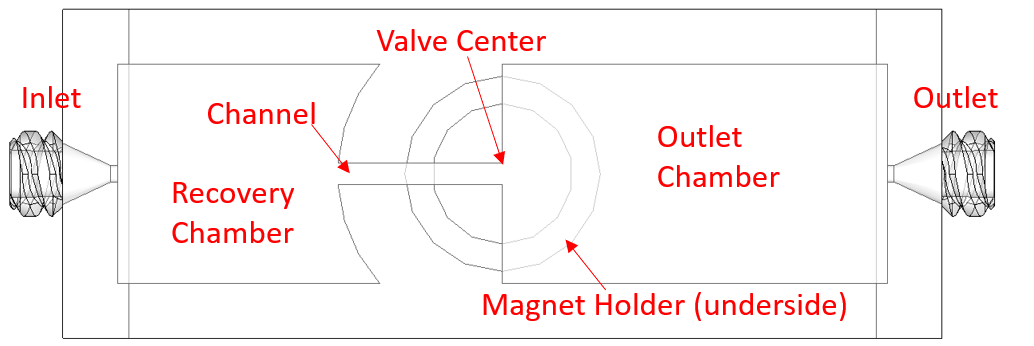
\includegraphics[width=3.34in]{figure/Figure1.png}}
\caption{The passive ferrofluid check valve components}
\label{fig_components}
\end{figure}
%%%%%%%%%%%%%%%% end figure %%%%%%%%%%%%%%%%%%%

The PFCV depicted in Fig.~\ref{fig_components} is a simple asymmetric volume
centered in a magnetic field
which holds a ferrofluid bolus in place.
In the center of a radially symmetric magnetic field
a narrow channel meets a larger open chamber at a right angle.
The ferrofluid bolus is large enough that at rest in the field it
forms a semi-circle in the open chamber. The narrow channel is
longer than the radius of the bolus at rest.
The broad chamber is the outlet side of the valve.
The narrow chamber opens onto a recovery chamber on the inlet
side of the valve.
This design allows the bolus to be recovered from the recovery
chamber when the pressure is equalized if the outlet pressure is
raised above the collapse pressure, driving the bolus away
from the magnetic field.
The PFCV does not resist pressure as well  as a
valve of the same size
made out of moving, solid parts.
That is, the sustainable
pressure it can resist on the outlet side before failing is relatively
low, and pressure required to crack it open and allow flow is
relatively high.
However, it may operate reliably within a range of
known pressures, and thus be sufficient to build a
pump-on-a-chip.
Furthermore, the PFCV reported here is a preliminary design which
can probably be significantly improved.
The authors found the
existence of the PFCV worth sharing immediately.

\section{Method}

The valve depicted Fig.~\ref{fig_components}
was designed using Solidworks 2016.
It is freely licensed via the CERN OHL Strong Reciprocal License\cite{stuckey2021,stuckey2021stl}.
The model consists of a 15mm long, 2mm wide channel, a large outlet
chamber, a recovery chamber,
two female luers, a magnet holder ring and two legs to provide room
for the magnet.  All volumes are 2mm high.
The 3D shape
of the chambers can be thought as a 2mm high extrusion of a 2D shape.
Viewed from the top, one end opens up to a recovery
chamber of circular profile 30mm in diameter and the other
an outlet chamber with a flat wall.
A magnet holder ring 12.7mm inner diameter (1/2'') was created centered on the channel-chamber
junction, below where the bolus is placed, to hold a permanent magnet in place
at the center of the valve. When two magnets are used, the magnet on
top naturally stays in the same position due to attraction to the magnet below.
On the inlet side of the channel
opens into a recovery chamber shaped to allow the ferrofluid to be
passively drawn back into the channel by the magnetic field after a
collapse of the bolus.
The model was printed on a Projet MJP 2500 (3D
Systems, Rock Hill, SC), using Visijet M2G-CL and VisiJet M2 SUP as
material and support respectively (3D Systems, Rock Hill, SC). Support
material was removed by using an EasyClean system (3D Systems, Rock
Hill, SC) and Dawn dish soap (Procter \& Gamble, Cincinnati, OH) to
remove residuals.


%%%%%%%%%%%%%%%% begin figure %%%%%%%%%%%%%%%%%%%
%%% 3.34in is the maximum width you can have for a figure
\begin{figure}
\centerline{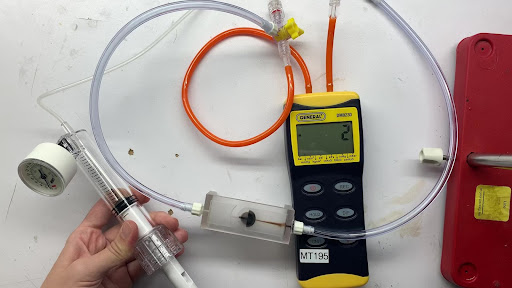
\includegraphics[width=3.34in]{figure/Figure2.jpeg}}
\caption{Equipment set up}
\label{fig_equipment}
\end{figure}
%%%%%%%%%%%%%%%% end figure %%%%%%%%%%%%%%%%%%%

As shown in Fig.~\ref{fig_equipment} and in our demonstration video\cite{stuckey2021video},
a basixCOMPAK 30atm pressurizing syringe (Merit Medical, South Jordan,
UT) is connected to the model via a two-way stopcock (Qosina,
Ronkonkoma, NY), tubing (Natvar, City of Industry, CA), and male
(Injectech, Fort Collins, CO) and female luer (Qosina, Ronkonkoma,
NY), allowing integration of a manometer (General Tools, Secaucus, NJ)
to measure pressure. A 12.7mm x 25.4mm (1/2” x 1”)
cylindrical neodymium magnet (Apex
Magnets, Petersburg, WV) with a pull force of 14.6 kg (32.24 pounds)
was placed inside the magnet channel by means
of a tight fit and 0.2 mL of ferrofluid (Apex Magnets, Petersburg, WV)
was injected into the model using a 3mL syringe (BH Supplies, Jackson,
NJ).

To obtain values, pressure was applied through the pressurizing
syringe, as demonstrated in a video \cite{stuckey2021video}.
Pressure was first applied from the outlet side of the model.
The maximum pressure difference from the outlet side that the
valve can withstand before collapsing, will be referred to as the
sustainable pressure or {\em collapse} pressure.
Pressure applied from the inlet needed to
initiate flow will be referred to as the {\em cracking} pressure.

The cracking pressure was first measured by increasing the pressure
difference on the inlet side until flow is initiated (at which point
the valve is ``open'' and
pushing the syringe plunger faster simply increases flow without
increasing the pressure.) Then the
collapse pressure was measured by increasing the pressure
difference on the outlet side. At pressures below the sustainable
pressure, the valve holds pressure well with no observable leaks of
air in the short time (a few minutes) of our experiment. When the
sustainable pressure is exceeded, the bolus explodes violently into
the recovery chamber. When the pressure difference is equalized, the
bolus may passively recover into the central position, or it may need
to be actively “combed” with a magnet back into the central position.

The procedure was performed first with one magnet, named the “Single
Magnet” configuration, placed below the channel-chamber connection.
The “Dual Magnet” configuration was performed with the magnet in the
same position as the Single Magnet case in the same position, but with
a second magnet of the same kind placed vertically on top of the model,
arranged to be strongly attracted to the lower magnet.

\section{Results}
The final pressures obtained demonstrate a clear difference between
the inlet cracking pressure and outlet sustainable pressure, creating
an effective passive check valve.

%%%%%%%%%%%%%%% begin table   %%%%%%%%%%%%%%%%%%%%%%%%%%
\begin{table}[t]
\footnotesize
\caption{Result pressures}
\begin{center}
\label{table_ASME}
\begin{tabular}{|p{0.3in} |p{0.4in} |p{0.49in} |p{0.45in} |p{0.6in} |}
\hline
Magnet configuration &
Cracking Pressure kPa  (mmHg) &
Collapse Pressure kPa  (mmHg) &
Pressure Difference kPa  (mmHg) &
Approx. Ratio: Cracking to Collapse Pressure \\
\hline
Single &
1.1 (8) &
5.5 (41) &
4.4 (33) &
1:5 \\
\hline
Dual &
8.5 (64) &
17.5 (131)&
8.9 (67)&
1:2 \\
\hline
\end{tabular}
\end{center}
\end{table}
%%%%%%%%%%%%%%%% end table %%%%%%%%%%%%%%%%%%%


The ferrofluid had observable differences in behavior between the two
configurations.  After the pressure equalized
following a collapse of the bolus due to
exceeding the sustainable pressure, the single magnet
configuration often repaired itself by drawing the fluid back
into a centered bolus passively.
After a collapse with two magnets, fluid further from the bolus
remained stationary while the fluid closer was pulled back to the
center. Following the removal of the top magnet, the stationary fluid
then began to return to the bolus. This is consistent with the
localization of the magnetic field between two magnets, and the
weakening of the magnetic field further from the channel-chamber
juncture in the dual magnet configuration.

Although the dual magnet configuration demonstrated a larger absolute
pressure difference due to magnetic field strength between the
cracking and the collapse pressure, the single magnet configuration
granted a larger ratio of collapse pressure to cracking
pressure due to the much lower cracking pressure.
The authors conjecture that the low cracking pressure may have
been not only to the weaker magnetic field, but the weakening at the
top of the 2mm high channel, which was further away from the magnet
in the single magnet configuration.

\section{Theory of Operation (Best as of Apr. 25)}

Let us consider an ideal blob of ferrfoluid.
\begin{itemize}
\item Assume that a blob in this section means an ideal 2-dimensional blob,
approximated by a blob constrained into a very thin plane.
\item Assume that the B-field is purely perpendicalur to this plane,
and that it completely dominates the magnetism induced in
the ferrofluid itself.
\item Assume that all forces of viscosity and surface tension may
  be ignored.
\item Although we will not model the forces that make it so,
  we will assume that blob of ferrofluid is self-connected and
  will not split into more than one blob.
\item The blob is perfectly incompressible, and so
  has an absolutely unchanging area.
\item The magnetic particles are evenly distributed in the
  fluid no matter what the magnetic field, so that the potential
  energy in the fluid by being in the field depends only on the
  strength of the field.
\item We need not treat the motion, velocity, or inertia of
  our fluid in any way.
\end{itemize}
Under suitable assumptions, we can state two drastically
simplifying assumptions.

\begin{conjecture}[Magnetostatic Blob Minimization]
  \label{conj:mbf}
  The magnetostaic force on an ideal 2-dimensional blob
  tends to minimize the potential energy in the blob
  and this occurs when its surfaces are in equal strength fields.
  Equivalently, every surface of a blob at rest with no outside
  forces is a line of equal field strength and all surfaces are equal.
\end{conjecture}


If the area is expanding the blob, it always decreases potential
energy. If the area is contracting the blob, it always increasing
potential energy. However, since the B-field at the two (or more)
surfaces may be different, there may be a force exerted on the
blob. In particular, we are interested in the force exerted on
the blob counterbalancing the force exerted on by fluid pressure
of non-ferrofluid at the surfaces.

Now imagine that a we have a monotone decreasing field centered
on the origin which which is not necessarily circular, with
the A region containg a thin tube, and the B region containing
a wide open region. Imagine that the field in B is radially
symmetric, but monotonically decreasing with distrance from
the origin (but not necessarily the same in the region A.)
A force resisting flow from the outlet to the inlet (from B to A)
is equal to the field strength at a point multiplied by the surface
length.
In this scenario, the air pressure on the blob is a function
of the length of the surface, but the magnetostatic force is
also a function of length, so the length cancels out and becomes
irrelevant.
The collapse pressure is therefore the maximum force at any point between the rest position and the origin
(this field is by construction equal on a semi-circular arc.)
The collapse pressure also depends on the field strength
at the point of the surface in A, but this surface has small length,
and therefore contributes little to the sum of the force.

Conversely, the cracking pressure will be minimized by
making the field strength in the region B as low as possible
at the point when the ferrfofuid has been entirely driven into
region A by air pressure from the inlet.

\subsection{How the Valve Cracks}

It is clear that a blob that has a bubble of non-ferrous fluid inside it
has higher potential energy that the same blob without that bubble.
Furthermore, such a bubble will feel a pressure to move away from
an area of a higher magnetic strength towared an area of weaker magnetic
strength. A bubble could be trapped, but if we assume that our
field decreases monotonically from a central peak, a bubble
will have a path to escape and will do so.
In this scenario a valve will ``crack'' that, is, crack open
allowing a fluid from the inlet to the outlet, as soon as the
non-ferrous fluid crosses a central boundary.

\subsection{Warmup: A Bolus in A Channel}

A relatively simple problem is to consider a bolus of
ferrofluid in thin channel. Placing a cylindrical permanent
magnet beneath it tends to lock the bolus in place.
If a small amount of air pressure is applied to from the West, the bolus will
be displaced to the East, but will find a stable point in balance with the
Westward forces exerted by the magnet.
As the pressure is increased, the bolus will be displaced futher Eastward.
It will reach a point where further displacement to the East does not increase
the Westward force, and will soon decrease it. At this point the plug will fail
catastrophically, spraying Eastward into the channel and letting air through.

The magnetic field in the line just above the face of the magnet can be analytically
described by ellpitical integrals, but they are very difficult to work with symbolically,
but easy to calculate numerically. MagPyLib is a convenient package for doing so.
Figure~\ref{fig:BolusSetup} shows our setup of the problem.

By making assumptions, we can
analyze this to obtain closed form solutions which match our
experience and inform more complicated cases.

\begin{figure}
\centerline{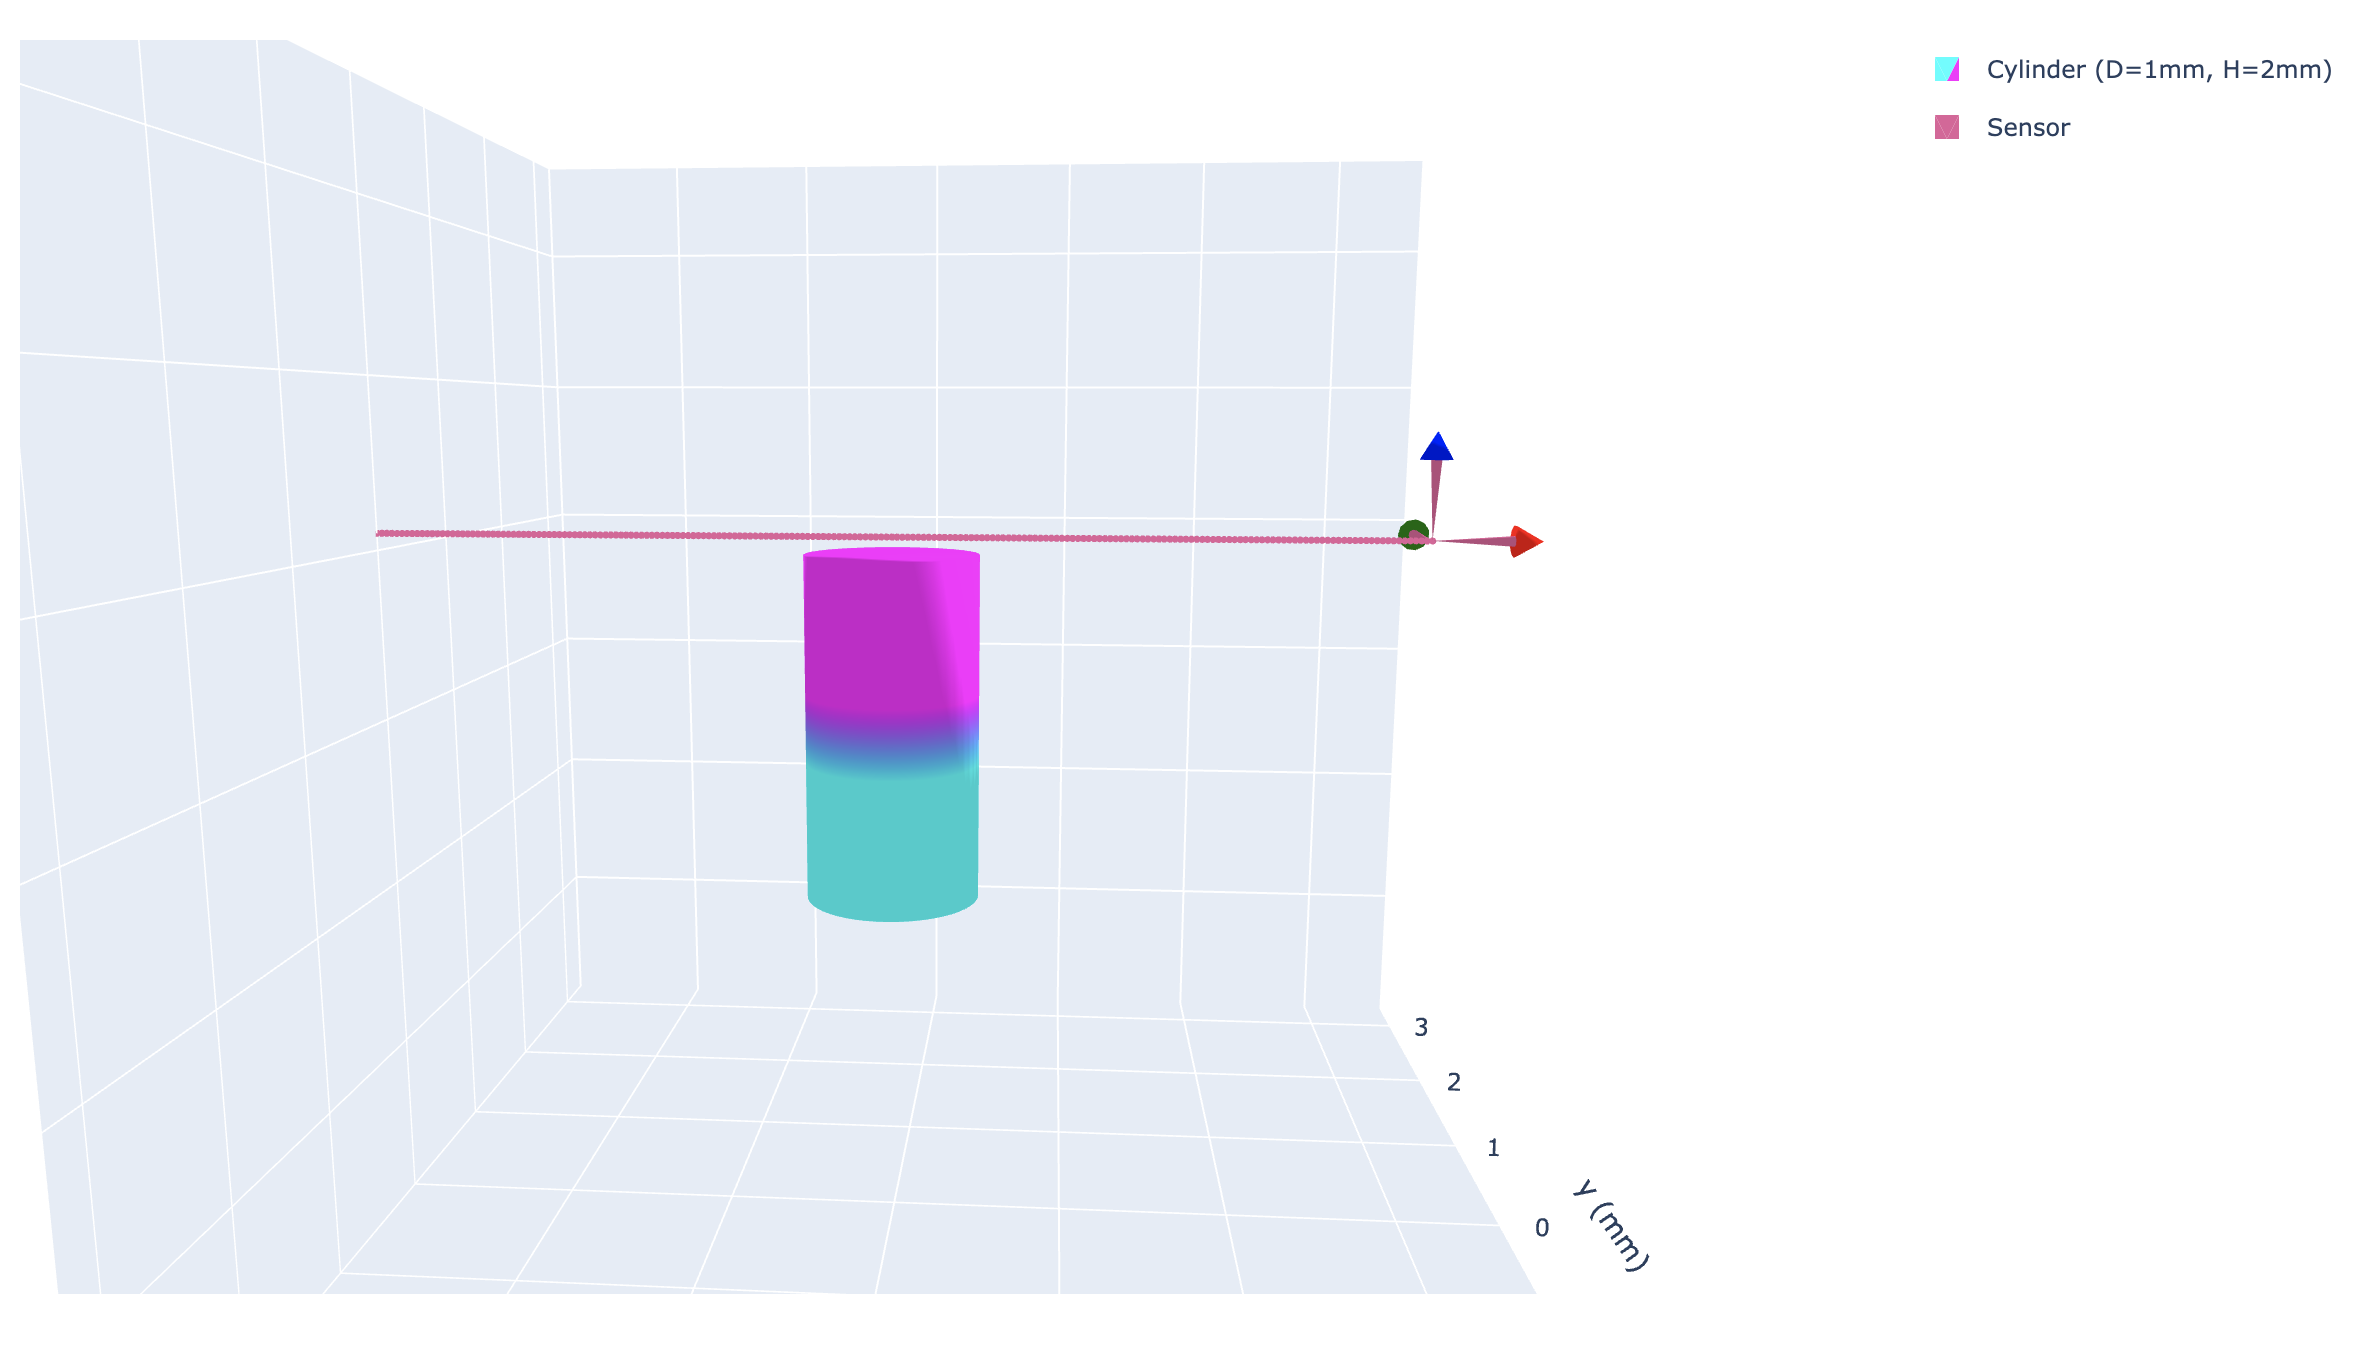
\includegraphics[width=6in]{figure/SetupBolusProblem.png}}
\caption{Setup of the Bolus Problem}
\label{fig:BolusSetup}
\end{figure}

The red line represents the thin channel just slightly above the face of
the magnet.
MagPyLib conveniently computes the field along this line. In particular,
only the $x$ component (the East-West coordinate) of the B-field is relevant to us.
The field was plotted with MagPyLib in Figure~ref{fig:Bx}. {\em Note: I do not understand the sign of this field. It appears to be wrong to me.}

\begin{figure}
\centerline{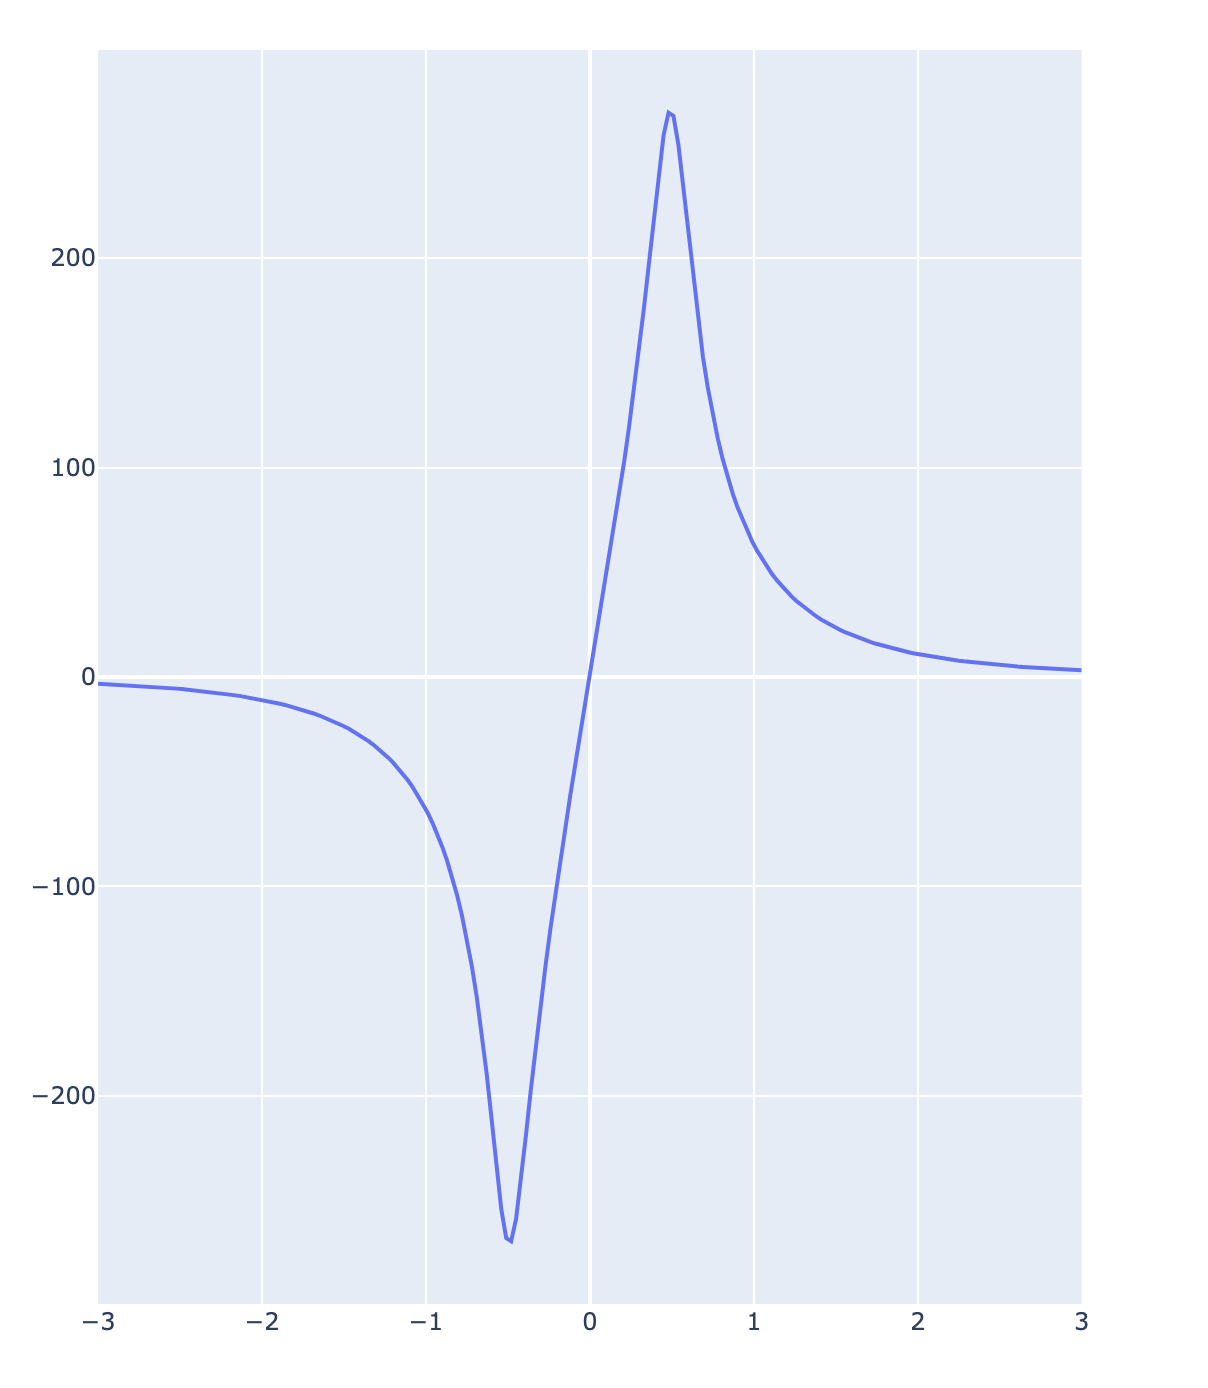
\includegraphics[width=3in]{figure/Bx.png}}
\caption{Bx component of field}
\label{fig:Bx}
\end{figure}

By inspection, we observe that this function can be accurately approximated with
a piecewise polynomial representation breaking the function at the extrema, which
are in fact the edges of the magnet. The resulting respresentation which is quadratic
to the West of the magnet, linear above the magnet, and quadratic East of the magnet
is remarkably accurate, under the assumption the MagPyLib is accurate. These
three approximations are shown in Figure~ref{fig:piecewise}.

\begin{figure}
\centerline{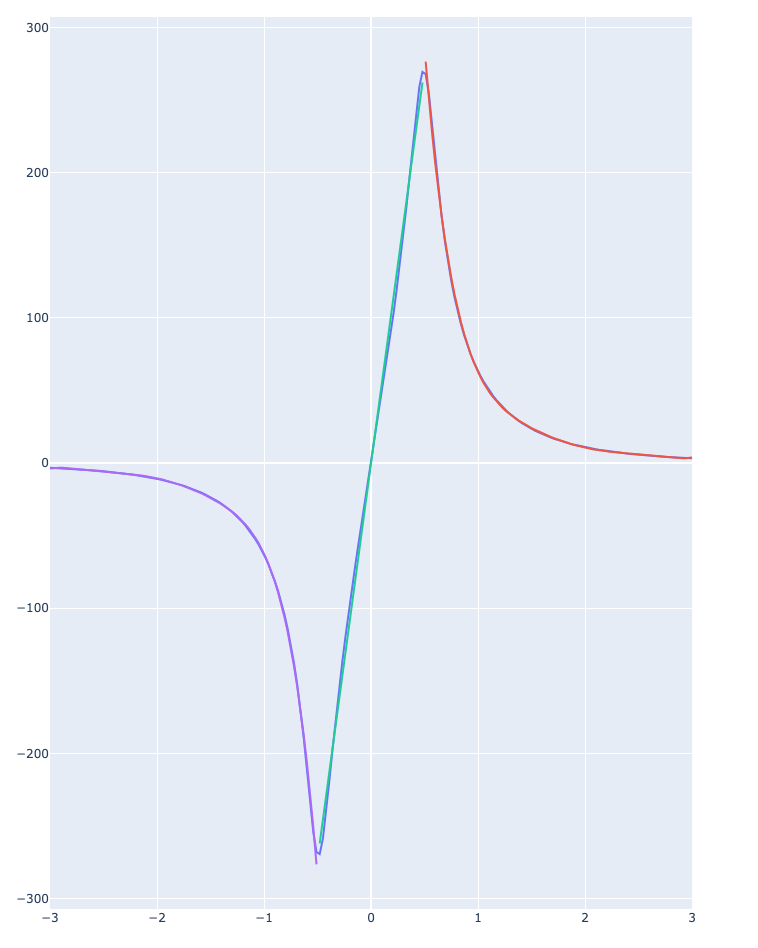
\includegraphics[width=3in]{figure/PlotOfBxWithPieceWiseInterpolation.png}}
\caption{Piecewise Representation of Field}
\label{fig:piecewise}
\end{figure}

The piecewise approximation $B'$ to the field $B$ is:

\begin{align}
  p(x) = & -18.5 x^6 + -230.2 x^5 + -1174.5 + \
  x^4 + -3154.6 x^3 + -4734.1 x^2 + -3819.4x + -1339.6 \\
  c(x) = & \hphantom{-}545.8 x \\
  q(x) = &  \hphantom{-}18.5 x^6 + -230.2 x^5 + \hphantom{-} 1174.5 + \
  x^4 + -3154.6x^3 +  \hphantom{-} 4734.1x^2 + -3819.4x + \hphantom{-} 1339.6 \\
B'(x) = &
\left\{
    \begin{array}{lr}
      0 , & \text{if } x < -3 \\
      p(x) , & \text{if } -3 < x  < -1/2 \\
      c(x) , & \text{if } -1/2 < x < 1/2 \\
      q(x) , & \text{if } 1/2 < x < 3 \\
      0 , & \text{if } x > 3
    \end{array}
    \right\}
    \label{eq:Bfield}
\end{align}

The numbers have been rounded to reflect the expected accuracy of the simulation and keep the expressions tractible.
It would be preferable to find these constants analytically from the
geometry and polarization of the magnet, but that is future work.

Where $P(x)$ and $Q(x)$ are nearly indentical 6-degree polynomials determined
by NumPy's polyfit.

The piecewise approximations: $p(x)$, $c(x)$, and $q(x)$ are
polynomials, which are easy to anti-differentiate to find the functions

$P,C$ and $Q$, such that $P' = p, C' = c,$ and $Q' = q$:

\begin{align}
  P(x) = & -1339.6 x - 1909.7 x^2 - 1578.03 x^3 - 788.65 x^4 - 234.9 x^5 - 38.3667 x^6 - 2.64286 x^7 \\
  C(x) = & 272.9 x^2 \\
  Q(x) = &  \hphantom{-}1339.6 x - 1909.7 x^2 + \hphantom{-}1578.03 x^3 - 788.65 x^4 + \hphantom{-}234.9 x^5 - 38.3667 x^6 + \hphantom{-}2.64286 x^7 \\
\end{align}





Setting aside issues of magnetic susceptibility of the ferrofluid used, the force is proportional
to the field strength times the area. Since the area is unchanging in a simple tube, the force on
a slice of ferrofluid at position $x$ is proportional to $B'(x)$.



Now imagine that bolus has a length of $L$, and let the channel area be $d$, and let $x$ be
the midpoint of the bolus.
Assume the magnet is a 1000 milliTesla (mT) polariazed magnet.
The $x$-axis force on the bolus can be computed as the integral of $dx$:

The $x$-axis force on a bolus in the channel centered at $y$ generally is proportional to:
\begin{align}
  F(y,L) = & \int_{y-L/2}^{y-L/2} B'(x) dx
\end{align}

Let us assume that we are blowing air from the left in the positive $x$ direction, in which case
we can ignore cases when $y < 0$. It is clear from symmetry that $ F(0,L) = 0 $ for any $L$.

\begin{align}
  F(y,L) = & \int_{y-L/2}^{y-L/2} B'(x) dx
\end{align}

In order to compute where the bolus will be when it explodes catastrophically when blown from
the negative $x$ direction to the positive $x$ direction, we simply need to know when the derirvative of
$F(y,L)$ with respect to $y$ becomes zero. Since $F(y,L)$ is a piecewise function, we can find $G(y,L)$,
integral of $F$ such that $d/dy G(y,L) = F(y,L)$. Let $D(x)$ be the integral of $B'(x)$.

\begin{align}
  D(x) =  &
\left\{
    \begin{array}{lr}
      0 , & \text{if } x < -3 \\
      P(x) , & \text{if } -3 < x  < -1/2 \\
      C(x) , & \text{if } -1/2 < x < 1/2 \\
      Q(x)   , & \text{if } 1/2 < x < 3 \\
      0 , & \text{if } x > 3
    \end{array}
    \right\}
    \label{eq:Dintegration}
\end{align}



Call the edge of the bolus blown in the positive $x$ direciton that has the lower $x$ value the high-side bolus and the edge with the higher $x$ value the low-side bolus.
This corresponds to the high-pressure side and the low-pressure side.

It is clear the collapse point will not occur until low-side edge is past greater than $1/2$. It is clear it will occur before the high-side edge reaches $1/2$. We therefore need only consider the bolus straddling
$1/2$.
Under these assumption, we have:
\begin{align}
  F(y,L) = & \int_{y-L/2}^{y+L/2} B'(x) dx \\
  F(y,L) = & \int_{y-L/2}^{0.5} c(x) dx  + \int_{0.5}^{y+L/2} q(x) dx   \\
  F(y,L) = & C(x) \bigg\rvert_{y-L/2}^{0.5}   +  Q(x) \bigg\rvert_{0.5}^{y+L/2} \\
  \begin{split}
  F(y,L) = & 272.9 0.5^2 - 272.9 (y-L/2)^2 + \\
  & 1339.6 (y+L/2) - 1909.7 (y+L/2)^2 + 1578.03 (y+L/2)^3 \\
  & - 788.65 (y+L/2)^4 + 234.9 (y+L/2)^5 - 38.3667 (y+L/2)^6 + 2.64286 (y+L/2)^7 \\
  & -(  1339.6 (0.5) - 1909.7 (0.5)^2 + 1578.03 (0.5)^3 \\
  & - 788.65 (0.5)^4 + 234.9 (0.5)^5 - 38.3667 (0.5)^6 + \\
  & 2.64286 (0.5)^7)
  \end{split} \\
  \begin{split}
  F(y,L) = & -278.875 - 272.9 (y-L/2)^2 + 1339.6 (y+L/2) - 1909.7 (y+L/2)^2 + \\
  & 1578.03 (y+L/2)^3 - 788.65 (y+L/2)^4 + 234.9 (y+L/2)^5 \\
  & - 38.3667 (y+L/2)^6 + 2.64286 (y+L/2)^7
  \end{split}
    \label{eq:force}
\end{align}

Using Wolfram alpha and setting $L = 1$, the maximum force occurs
at $y = 0.592, F \propto 142.4 $, when the center of the bolus is just to the right
of the break point. This accords with the graph inspection.

At $L = 2.0$, $y = 1.01766, F \propto 167.07$.


\subsection{The Channel-to-a-Chamber}

Our goal, however, is to analyze a somewhat more complicated geometry.
In particular, we are interested in a channel-leading-to-a-chamber,
as depicted in Fig.~\ref{fig:ChannelToChamber}.

\begin{figure}
\centerline{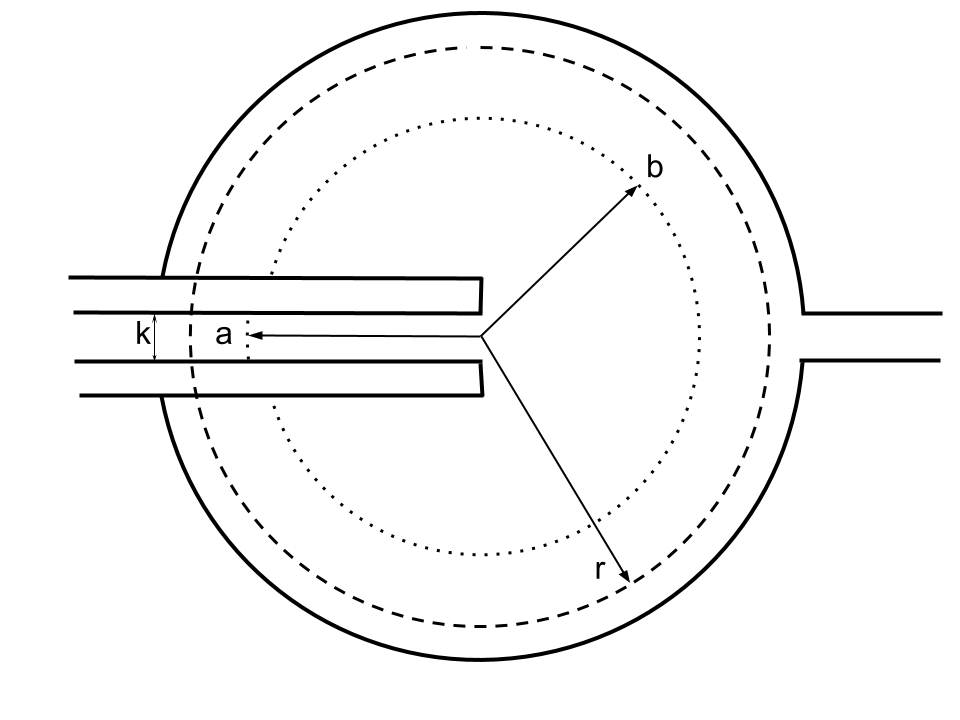
\includegraphics[width=4in]{figure/ChannelToChamber.png}}
\caption{Channel To Chamber Geometry}
\label{fig:ChannelToChamber}
\end{figure}

We would ideally like to treat this as a one-dimensional problem as well.
Let us assume once again that a magnetic field is placed at the center
at our diagram (where the channel meets the chamber.)
Call the region to the left A and the region to the right B, and assume
the orgin is at the center of the diagram.

The most important geometric feature of the channel-and-chamber
valve design is the radius of the cylindrical magnet or magnets
in it. It will be most convenient to take the radius of this
magnet to be unity (1.0) and express all other spatial
measures relative to that. The origin of our plane of operation
will be the center of the top face of the cylindrical magnet,
which is assumed to be beneath the plane, with its North face
in contact with the plane.

Note: I believe using a magnetic force that falls off with the square of distance may
not allow for a stable solution. I am not sure how to model this in a way
which is realistic and convenient. Using the fourth power will probably work and
may be realistic given of action is perpendicular to the magnet. I think I will try it.

In what follows, region $A$ is the inlet region and region $B$ is the
outlet region; I should probably remove the labels $A$ and $B$ entirely
since we are using $B$ for the B-field.

Let us assume once again a magnetic field centered on the origin as generated by a
1/2'' by 1'' cylindrical magnet as defined by Equation~ref{eq:Bfield}.
Since that field is completely radially symmetric, we can use that equation to
describe the B field in the plane, where the parameter of the function
is the distance from the center of the face of the magnet.



Since we have previously assumed that the bolus is a single blob,
at least until it collapses, then we can can relate $a$ and $b$
via the total area of the bolus $S$.
Let us assume that the channel of width $d$ is narrow enough
that the slight arc of the fluid inside the inlet region can be treated as a
straight line.
\begin{align}
S = d \cdot a + \frac{1}{2} \pi b^2
\end{align}
when $a > 0$ and $b > 0$, so that the areas of $A$ and $B$ are both positive.
It is most convenient to measure our position of the bolus, which is
changing shape in this case, as the coordinate $b$, so we we express
$a$ in terms of $b$. Since we will use this algebraic relationship later, we will define it as a function $A$:
This can be solved for $a$:
\begin{align}
  a = A(b) = -\frac{\pi b^2 - 2 S}{2d}
  \label{eqn:afromS}
\end{align}


Note that when $a = 0$, the dependence on $d$ vanishes and:
\begin{align}
  b = & \sqrt{\frac{2S}{\pi}} \\
  b^2 = & \frac{2S}{\pi}
  \label{eq:a_zero}
\end{align}

Since at rest the bolus surface $A$ will be in the same field strength as surface $B$, we can set:

\begin{align}
  B(a) = & B(b) \\
  B(-\frac{\pi b^2 - 2 S}{2d}) = & B(b)
\end{align}

This can be solved by WolframAlpha (results not incuded here.)
As expected, $ b = -a $, that is, both surfaces are equidistant from the
center of our radially symmetric magnetic field.

\subsection{A strategy for computing pressure}

Our fundamental goal is to compute the collapse and cracking
pressure. The collapse pressure is determined by the maximum force needed
to reduce $b$ in the outlet region past some point we will call the
{\em collapse point.}
The cracking pressure is the pressure needed to drive the region $A$, represented
by the variable $a$, to the {\em cracking point}, at which point
a bubble forms and is pushed to the outlet.

The check valve we are trying to design will be characterized by
both the collapse pressure and the cracking pressure, but in a single
number the can define the performance of the valve as this ratio $P$,
which we want to be as high as possible:
\begin{align}
  P = \frac{\text{Collapse Pressure}}{\text{Crack Pressure}}
  \end{align}

If the bolus at rest is displaced, the potential energy increases,
moving off a minimum. At a given point, the infinitessimal change
in energy divided by the infinitessimal change in distance
is equal to the force.

If we had a formula for the potential energy as a function of $b$,
we would have a chance of computing this analytically.

In this model, which is using a the narrowness of the plane to simplify
the problem. In this simplified model, we can assume
that the potential energy of the magnetic system can be simply
modeled by the presence or absence of ferrofluid at a point in the plane.
The presence of ferrofluid at a point or infinitessimal area ($da$) decreases the potential energy $U$
of the entire system in proportion to the strength of the field at a point,
and that that strength is describe by our function $B(r)$ where $r$ is the
distance from the origin (and thus the center of the face of the magnet).
We can thus describe the potential energy as an integral over surface patches:

\begin{align}
  U = -\int
\left\{
    \begin{array}{lr}
      B(a)  , & \text{if there is ferrofluid at } a \\
      0 , & \text{if there is no ferrofluid at } a
    \end{array}
\right\} da
\end{align}

We are furthermore ignoring all effect of the ferrofluid interacting with itself in terms
of the potential energy. However, we rely on the very important property of ferrofluid that
it tends to clump together into a single blob in the presence of a magentic field.
We will, in fact, assume that our blob or bolus is perfectly hemispherical in the chamber,
and a perfect rectangle in the channel. Furthermore, we assume the fluid is incompressible,
and therefore always as the aread $S$. This is true until the bolus collapses; we know that
when it collapses it explodes drastically, and we do not attempt to model anything after
a collapse event.

Therefore, we in fact have a one dimensional system of the coordinate $b$, which
it is convenent to break into $U = U_A + U_B$. We assume that the channel $A$ is narrow
enough that we can model the field across the channel as if it is rectilinear.

\begin{align}
  U_A = & -\int_0^b B(r) dr , & \text{if } -pi/2 < \theta < pi/2 \\
  U_A = & -\pi \int_0^b B(r) dr \\
  U_B = & -d \int_0^a B(r) dr\\
\end{align}

However, we have previously computed the indefinite integral $D(x) = \int B(x)$ in Equation~\ref{eq:Dintegration},
so:
\begin{align}
  U = & -\pi D(x) \vert_{x=0}^{x=b}  + -d D(x)\vert_{y=0}^{y=A(b)} \\
  U = & -\pi (D(b) - D(0)) + -d (D(A(b)) - D(0))
\end{align}

We can use this expression, if we can differentiate it, to compute force necessary to displace the bolus to one side or another:
\begin{align}
  dU = -F_r dr
\end{align}

But before attempting that, we simply observe that the bolus will will collapse when the force on
it caused by pressure from the right (in the chamber) drives it to the point where the force
resiting it is maximized.

Qualitatively, we assume that at rest (ambient pressure), the bolus exerts no force. As the
pressure in the chambe increases, the force (the change in potential energy) will increase
as $b$ is decreased and the bolus is disturbed from its rest position. This force will increase
as $b$ decreased further from its rest postion. However, eventuall this force will cease to
increase and reach its maximum. At that point, the valve will collapse.

Our strategy is thus to find the value of $b$ $b_m$ that maximizes the force (maximizes the change in
potential energy $dU$). The force at $b_m$, $F(b_m)$ will be equal to the pressure times $\pi b_m$, and
that will be the collapse pressure $P_c$.

\begin{align}
  F(b_m) = & \pi b_m P_c \\
  P_c = \frac{F(b_m)}{\pi b_m}
\end{align}

The cracking pressure $P_r$ will be the force necessary to reach $a = 0$, because at that point,
the non-magnetic fluid will form a ``bubble'' which will be pinched off and displaced into the chamber
by the ferrofluid. This ``bubble'' will be forced in the direction of decreasing mangentic field strength,
because it minimizes potential energy to fill the strong field with ferrofluid preferentially over
non-magnetic fluid. This occurs at $a = 0$, so $A(b) = 0$, or $b = \sqrt{\frac{2S}{\pi}}$ by Equation~\ref{eq:a_zerio}.

\begin{align}
  P_r d = F(\sqrt{\frac{2S}{\pi}})
\end{align}


\subsection{Conjecture}

Important note: This math strongly suggest that the valve can be
made twice as performant by opening the chamber completely, so that the
valve is merely a chamber in the center of the bolus.
Likewise thickening of the chamber (in the z-dimesion, violating
our current 2-dimensional assuption) at the point of the strongest
magent force would mean that more ferrofluid would have to be driven
away at that point, increasing the potentially energy and therefore
requiring more force.

However, even though we have modeled the fluid as not reacting to itself,
we would not want the ferrofluid itself
to strengthen the field on the inlet side, which might occur. Creating
therefore an arc of someething less than 360 degrees, such as 270 degrees,
or making the walls of the thin chamber very thick, might solve this problem.

This math makes it clear that on the outlet side we want the
bolus surface to be outside a strong field at $r$ to that $r B(r)$ is
maximized to maximize the collapse pressure.
Let us call the value of $b$ that maximizes $b B(b)$ the {\em collapse point.}
We can now see that we want $S$ to be large enough that the edge
of the bolus at rest is beyond the collapse point by some
comfortable margin.

However, to minimize the crack pressure, we want the bolus at rest
in the region $A$ inside
the collapse point, because we don't want the inlet pressure to have
to overcome that, even though on the inlet side the length $d$ will
be much smaller that length $\pi b$. However, by the
Magnestatic Blob Minimization principle, this is impossible in a
radially symmetric B field.

This suggest that on the inlet side we attempt to make
the magnetic field, only within the channel, as gradual, linear, and
long as possible. This might be possible to accomplish by simply adding
a piece of ferrous metal under the channel, or by making the channel
itself a steel needle. A specially designed magnet or two magnets could be
used. This is somewhat depicted in Fig.~\ref{fig:ifp}.

\begin{figure}
\centerline{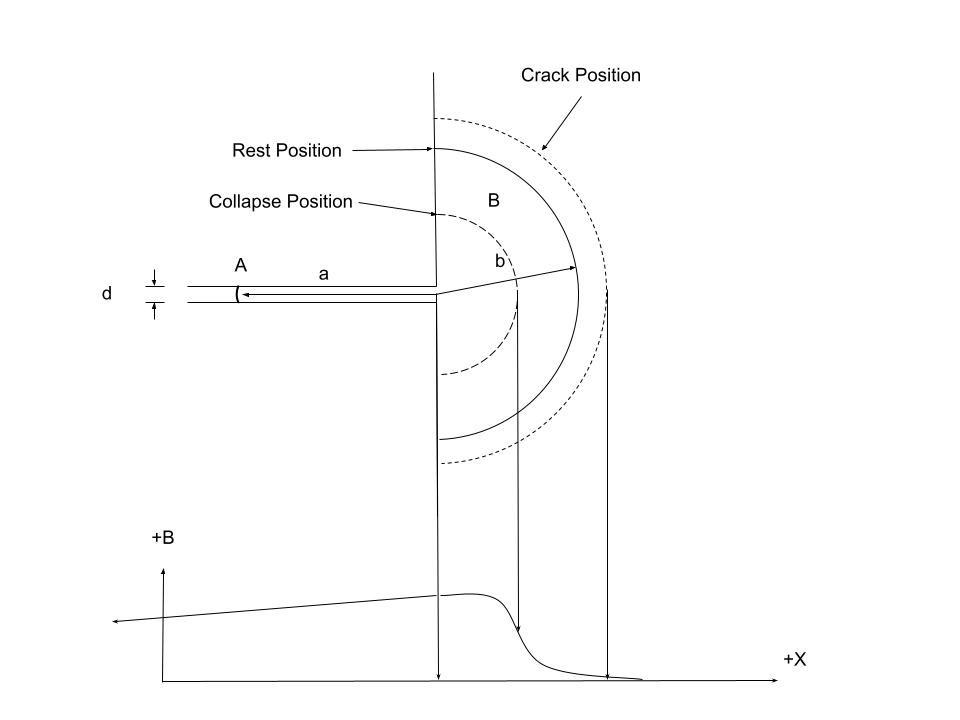
\includegraphics[width=6in]{figure/IdealFieldProfile.png}}
\caption{(Rough) Ideal Field Profile}
\label{fig:ifp}
\end{figure}

\subsection{Idea: An Improved Version}

It is clear based on the above theory that allowing the bolus to be semi-circular
is an arbitrary inefficiency. There is no reason not to allow a 360 degree bolus,
as depicted in Figure~\ref{fig:360}.

\begin{figure}
\centerline{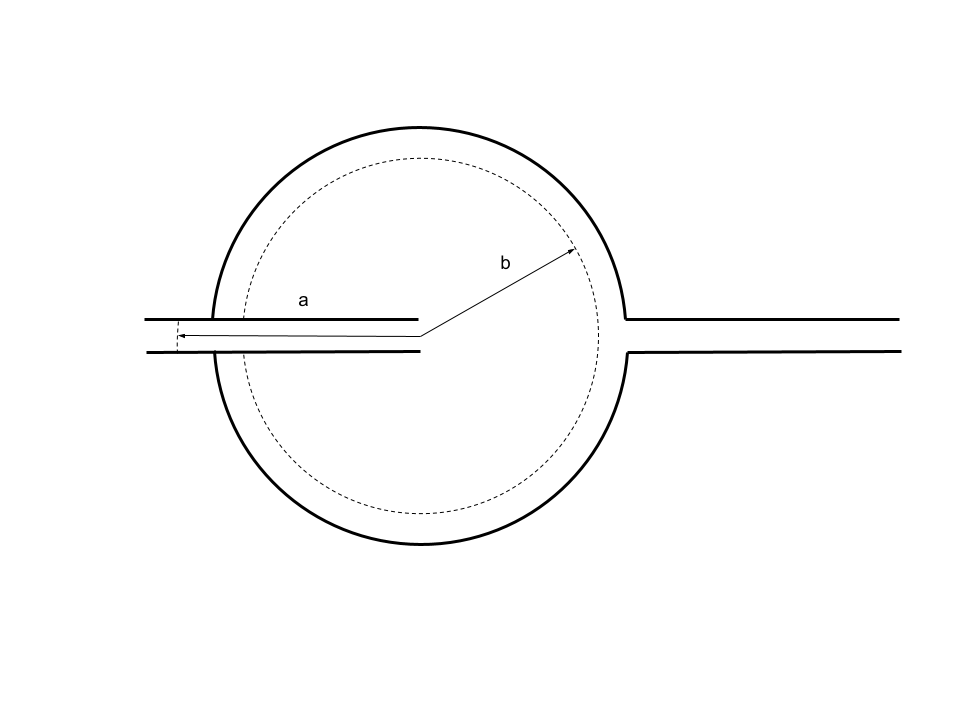
\includegraphics[width=6in]{figure/360degreeplanarcheckvalve.png}}
\caption{360 degree planar check valve, an improvement derived from theory}
\label{fig:360}
\end{figure}

\subsection{Idea: a 3D version}

It if we had a very powerful and very small dipole, it could in theory
collect a complete sphere of ferrofluid around it. Possibly the tip
of a conical magnet would nearly do this.
In a spherical-like magnetic field, the same principle would
apply, but the added dimensionality would be expected to further
separate the collapse pressure from the crack pressue.

However, a simpler version of this idea based on accessible
cylindrical bar magnets is depicted in Fig.~\ref{fig:3dcheckvalve}.
This has not yet been experimentally tested.

The advantage of having a 3D version predicted by the math is that the area
of the small inlet port would be tiny compared to the area of the spherical
shape. This would tend to produce a very performant valve, if the magnet
field can be designed with sufficient strength. It would seem to be harder
to manufacture in the intended use case of very small valves.

There are two obvious ways to manufacture such a 3D device, both of which require
drilling a small hole into magnet. The first is use a small cylidrical or spherical
magnet. This would be a dipole that could not be approximated as a radially
symmetric field; but it might work anyway.  The second would be to drill a hole
through the axis of a conical magnet. Hopefully the concentration of field strength
at the apex of the magnet would produce a roughly spherical field strength.

Possibly rather than using a sphere, a hemisphere would be more reasonable.

\begin{figure}
\centerline{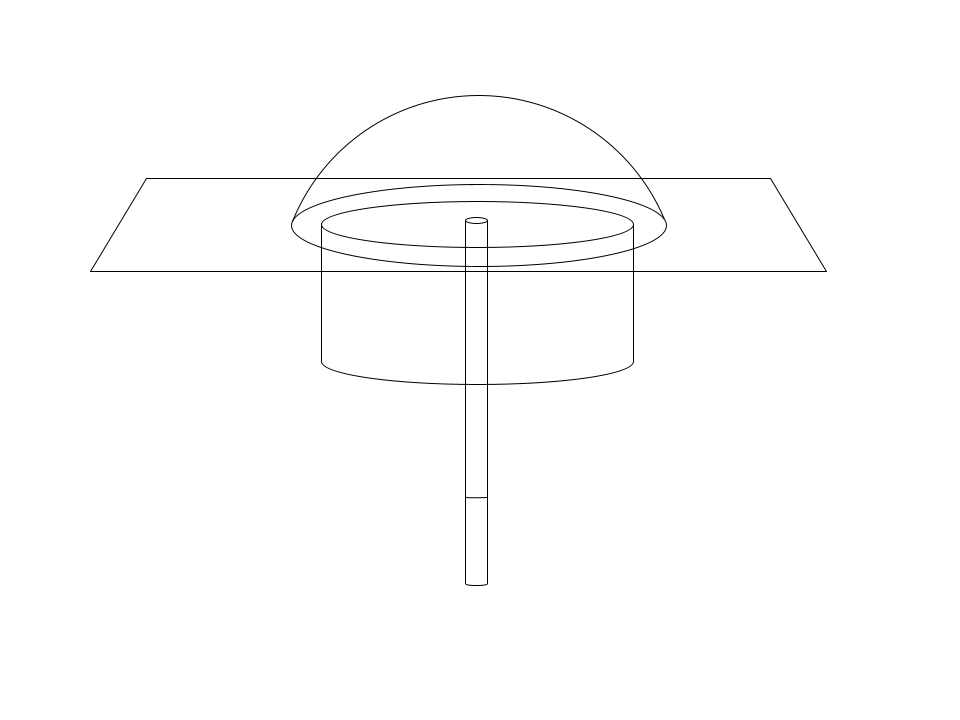
\includegraphics[width=6in]{figure/3DCheckValve.png}}
\caption{Untested 3D check valve idea}
\label{fig:3dcheckvalve}
\end{figure}

\subsection{Idea}

We can protect the valve from explosive collapse by using a separate
valve that cracks before the collapse pressure, acting as a ``pop-off''
valve.





\section{Conclusions}

This paper demonstrates an apparently novel passive ferrofluid one-way
valve or check valve (PFCV). This valve is completely passive in that
it depends entirely on the pressure at the inlet port and the outlet
port. The valve has no moving parts (except for the ferrofluid, which
is almost stationary), and a remarkably simple design, consisting of
nothing but a channel, an inlet chamber, and outlet chamber,
and a bolus of ferrofluid in a
static magnetic field.

Although no effort has been made to optimize the design, the pressure
difference between the cracking pressure and the sustainable back
pressure appear great enough to make an effective micropump. The
performance of this one-way valve may improve with additional design
effort; the authors sought to publish this result as soon as it was
observed.  Obvious future research possibilities are:
\begin{enumerate}
\item  To improve the
performance by varying the geometry of the passive design or shape and
strength of the magnetic field.
\item Utilizing this design to make a micro-pump
similar to earlier micro-pumps but with this simpler check valve
design.
\item To provide an explanatory and predictive theory of operation,
for example based on magnetic field strength as per \cite{ando2009ferrofluidic}.
\item Studying the ability of the valve to recover after
  a collapse automatically when high outlet pressure is removed,
  which would increase robustness in some applications.
\end{enumerate}

%%%%%%%%%%%%%%%%%%%%%%%%%%%%%%%%%%%%%%%%%%%%%%%%%%%%%%%%%%%%%%%%%%%%%%
% The bibliography is stored in an external database file
% in the BibTeX format (file_name.bib).  The bibliography is
% created by the following command and it will appear in this
% position in the document. You may, of course, create your
% own bibliography by using thebibliography environment as in
%
% \begin{thebibliography}{12}
% ...
% \bibitem{itemreference} D. E. Knudsen.
% {\em 1966 World Bnus Almanac.}
% {Permafrost Press, Novosibirsk.}
% ...
% \end{thebibliography}

% Here's where you specify the bibliography style file.
% The full file name for the bibliography style file
% used for an ASME paper is asmems4.bst.
\bibliographystyle{asmems4}

% Here's where you specify the bibliography database file.
% The full file name of the bibliography database for this
% article is asme2e.bib. The name for your database is up
% to you.
\bibliography{asme2e}

\end{document}

%%%%%%%%%%%%%%%%%%%%%%%%%%%%%%%%%%%%%%%%%%%%%%%%%%%%%%%%%%%%%%%%%%%%%%
\appendix       %%% starting appendix
\section*{Appendix A: Head of First Appendix}
Avoid Appendices if possible.

%%%%%%%%%%%%%%%%%%%%%%%%%%%%%%%%%%%%%%%%%%%%%%%%%%%%%%%%%%%%%%%%%%%%%%
\section*{Appendix B: Head of Second Appendix}
\subsection*{Subsection head in appendix}
The equation counter is not reset in an appendix and the numbers will
follow one continual sequence from the beginning of the article to the very end as shown in the following example.
\begin{equation}
a = b + c.
\end{equation}

%%%%%%%%%%%%%%%%%%%%%%%%%%%%%%%%%%%%%%%%%%%%%%%%%%%%%%%%%%%%%%%%%%%%%%
\subsection{Second-Level Heading}

The next level of heading is also boldface with upper and lower case letters.
The heading is flushed left with the left margin. The spacing to the next heading is two line spaces.

%%%%%%%%%%%%%%%%%%%%%%%%%%%%%%%%%%%%%%%%%%%%%%%%%%%%%%%%%%%%%%%%%%%%%%
\subsubsection{Third-Level Heading.}

The third-level of heading follows the style of the second-level heading.


%%%%%%%%%%%%%%%%%%%%%%%%%%%%%%%%%%%%%%%%%%%%%%%%%%%%%%%%%%%%%%%%%%%%%%
\section{Use of SI Units}

An ASME paper should use SI units.  When preference is given to SI units, the U.S. customary units may be given in parentheses or omitted. When U.S. customary units are given preference, the SI equivalent {\em shall} be provided in parentheses or in a supplementary table.

%%%%%%%%%%%%%%%%%%%%%%%%%%%%%%%%%%%%%%%%%%%%%%%%%%%%%%%%%%%%%%%%%%%%%%
\section{Footnotes\protect\footnotemark}
\footnotetext{Examine the input file, asme2ej.tex, to see how a footnote is given in a head.}

Footnotes are referenced with superscript numerals and are numbered consecutively from 1 to the end of the paper\footnote{Avoid footnotes if at all possible.}. Footnotes should appear at the bottom of the column in which they are referenced.


%%%%%%%%%%%%%%%%%%%%%%%%%%%%%%%%%%%%%%%%%%%%%%%%%%%%%%%%%%%%%%%%%%%%%%
\section{Mathematics}

Equations should be numbered consecutively beginning with (1) to the end of the paper, including any appendices.  The number should be enclosed in parentheses and set flush right in the column on the same line as the equation.  An extra line of space should be left above and below a displayed equation or formula. \LaTeX\ can automatically keep track of equation numbers in the paper and format almost any equation imaginable. An example is shown in Eqn.~(\ref{eq_ASME}). The number of a referenced equation in the text should be preceded by Eqn.\ unless the reference starts a sentence in which case Eqn.\ should be expanded to Equation.

\begin{equation}
f(t) = \int_{0_+}^t F(t) dt + \frac{d g(t)}{d t}
\label{eq_ASME}
\end{equation}

%%%%%%%%%%%%%%%%%%%%%%%%%%%%%%%%%%%%%%%%%%%%%%%%%%%%%%%%%%%%%%%%%%%%%%
\section{Figures}
\label{sect_figure}

All figures should be positioned at the top of the page where possible.  All figures should be numbered consecutively and centered under the figure as shown in Fig.~\ref{figure_ASME}. All text within the figure should be no smaller than 7~pt. There should be a minimum two line spaces between figures and text. The number of a referenced figure or table in the text should be preceded by Fig.\ or Tab.\ respectively unless the reference starts a sentence in which case Fig.\ or Tab.\ should be expanded to Figure or Table.


%%%%%%%%%%%%%%%%%%%%%%%%%%%%%%%%%%%%%%%%%%%%%%%%%%%%%%%%%%%%%%%%%%%%%%
%%%%%%%%%%%%%%%% begin figure %%%%%%%%%%%%%%%%%%%
\begin{figure}[t]
\begin{center}
\setlength{\unitlength}{0.012500in}%
\begin{picture}(115,35)(255,545)
\thicklines
\put(255,545){\framebox(115,35){}}
\put(275,560){Beautiful Figure}
\end{picture}
\end{center}
\caption{The caption of a single sentence does not have period at the end}
\label{figure_ASME}
\end{figure}
%%%%%%%%%%%%%%%% end figure %%%%%%%%%%%%%%%%%%%
%%%%%%%%%%%%%%%%%%%%%%%%%%%%%%%%%%%%%%%%%%%%%%%%%%%%%%%%%%%%%%%%%%%%%%

In the following subsections, I have inserted figures that have been provided by authors in order to demonstrate what to avoid.  In each case the authors provided figures that are 3.25in wide and 600dpi in the .tif graphics format.  The papers containing these figures have been held from production due to their poor quality.

%%%%%%%%%%%%%%%%%%%%%%%%%%%%%%%%%%%%%%%%%%%%%%%%%%%%%%%%%%%%%%%%%%%%%%
\subsection{The 1st Example of Bad Figure}

%%%%%%%%%%%%%%%% begin figure %%%%%%%%%%%%%%%%%%%
%%% 3.34in is the maximum width you can have for a figure
\begin{figure}
\centerline{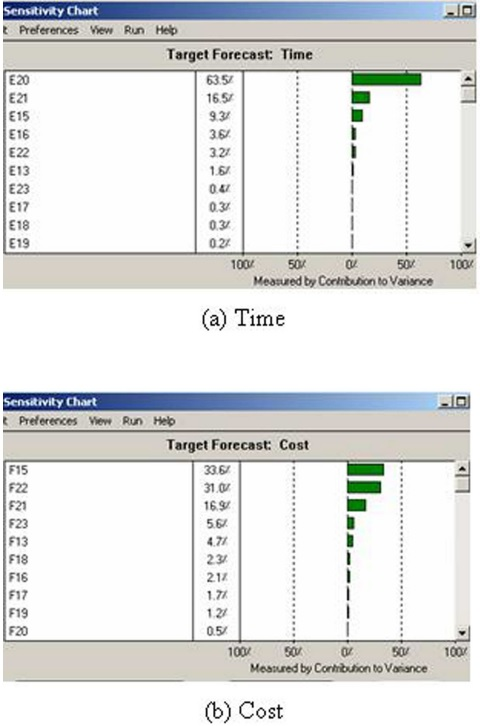
\includegraphics[width=3.34in]{figure/FMANU_MD_05_1107_11.jpg}}
\caption{Example taken from a paper that was held from production because the image quality is poor.  ASME sets figures captions in 8pt, Helvetica Bold.}
\label{fig_example1.jpg}
\end{figure}
%%%%%%%%%%%%%%%% end figure %%%%%%%%%%%%%%%%%%%

In order to place the figure in this template using MSWord, select Insert Picture from File, and use wrapping that is top and bottom. Make sure the figure is 3.25in wide.

Figure~`\ref{fig_example1.jpg}
was taken from a recent paper that was held from publication, because the text is fuzzy and unreadable. It was probably obtained by taking a screen shot of the computer output of the authors software. This means the original figure was 72dpi (dots per inch) on a computer screen. There is no way to improve the quality such a low resolution figure.

In order to understand how poor the quality of this figure is, please zoom in slightly, say to 200\%.  Notice that while the font of the paper is clear at this size, the font in the figures is fuzzy and blurred.  It is impossible to make out the small symbol beside the numbers along the abscissa of the graph.  Now consider the labels Time and Cost. They are clearly in fonts larger that the text of the article, yet the pixilation or rasterization, associated with low resolution is obvious. This figure must be regenerated at higher resolution to ensure quality presentation.

The poor quality of this figure is immediately obvious on the printed page, and reduces the impact of the research contribution of the paper, and in fact detracts from the perceived quality of the journal itself.



%%%%%%%%%%%%%%%%%%%%%%%%%%%%%%%%%%%%%%%%%%%%%%%%%%%%%%%%%%%%%%%%%%%%%%
\subsection{The 2nd Example of Bad Figure}

%%%%%%%%%%%%%%%% begin figure %%%%%%%%%%%%%%%%%%%
\begin{figure}
\centerline{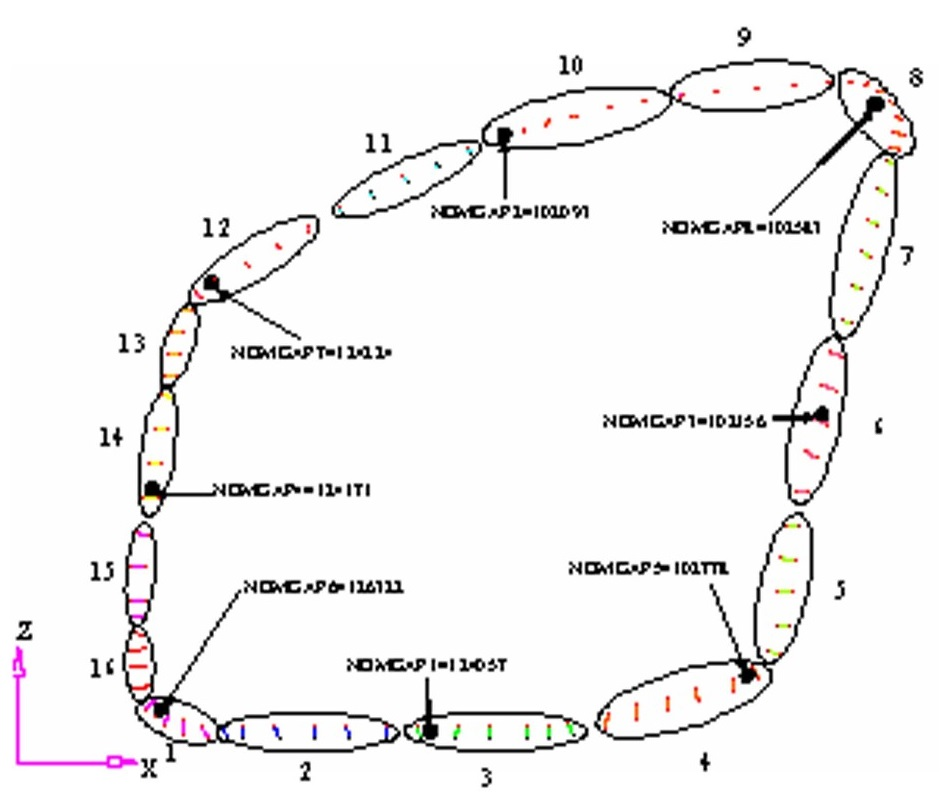
\includegraphics[width=3.34in]{figure/FMANU_MD_05_1272_5.jpg}}
\caption{While this figures is easily readable at a double column width of 6.5in, when it is shrunk to 3.25in column width the text is unreadable. This paper was held from production.}
\label{fig_}
\end{figure}
%%%%%%%%%%%%%%%% end figure %%%%%%%%%%%%%%%%%%%

Figure~\ref{fig_example2.jpg}
demonstrates a common problem that arises when a figure is scaled down fit a single column width of 3.25in.  The original figure had labels that were readable at full size, but become unreadable when scaled to half size.  This figure also suffers from poor resolution as is seen in the jagged lines the ovals that form the chain.

This problem can be addressed by increasing the size of the figure to a double column width of 6.5in, so the text is readable.  But this will not improve the line pixilation, and a large low resolution figure is less desirable than a small one.  This also significantly expands the length of the paper, and may cause it to exceed the JMD nine page limit.  Additional pages require page charges of \$200 per page.  It is best to regenerate the figure at the resolution that ensures a quality presentation.


%%%%%%%%%%%%%%%%%%%%%%%%%%%%%%%%%%%%%%%%%%%%%%%%%%%%%%%%%%%%%%%%%%%%%%
\subsection{The 3rd Example of Bad Figure}
%%%%%%%%%%%%%%%% begin figure %%%%%%%%%%%%%%%%%%%
\begin{figure}
\centerline{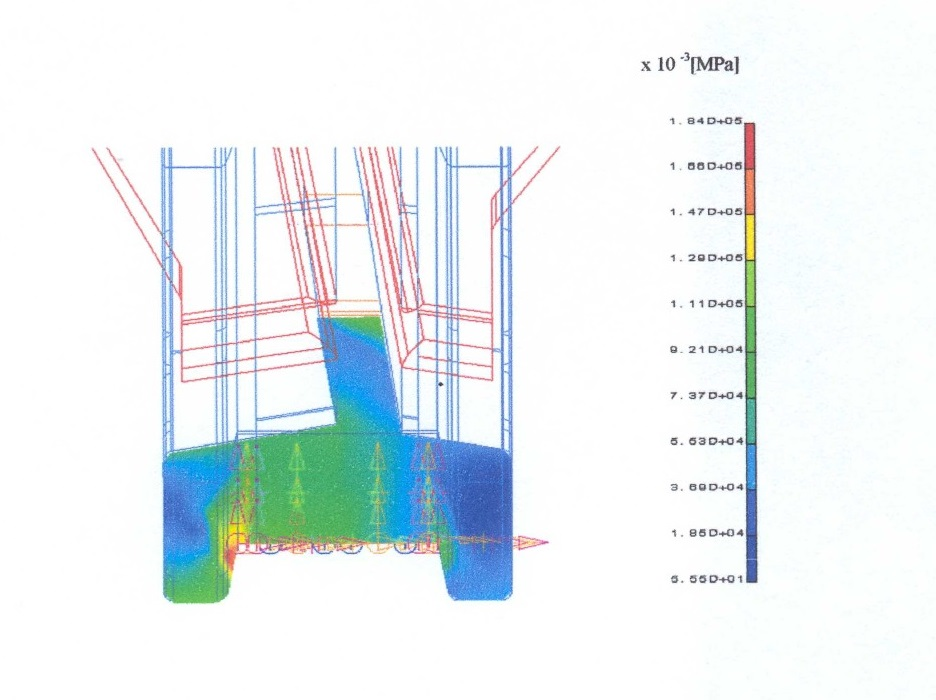
\includegraphics[width=3.25in]{figure/FMANU_MD_04_1274_13.jpg}}
\caption{Another example of a figure with unreadable text.  Even when the paper was expanded to double column width the text as shown in Fig.~\ref{fig_example4.jpg} was of such low quality that the paper was held from production.}
\label{fig_example3.jpg}
\end{figure}
%%%%%%%%%%%%%%%% end figure %%%%%%%%%%%%%%%%%%%

%%%%%%%%%%%%%%%% begin figure %%%%%%%%%%%%%%%%%%%
%%% the maximum width in double column is 6.85in
\begin{figure*}
\centerline{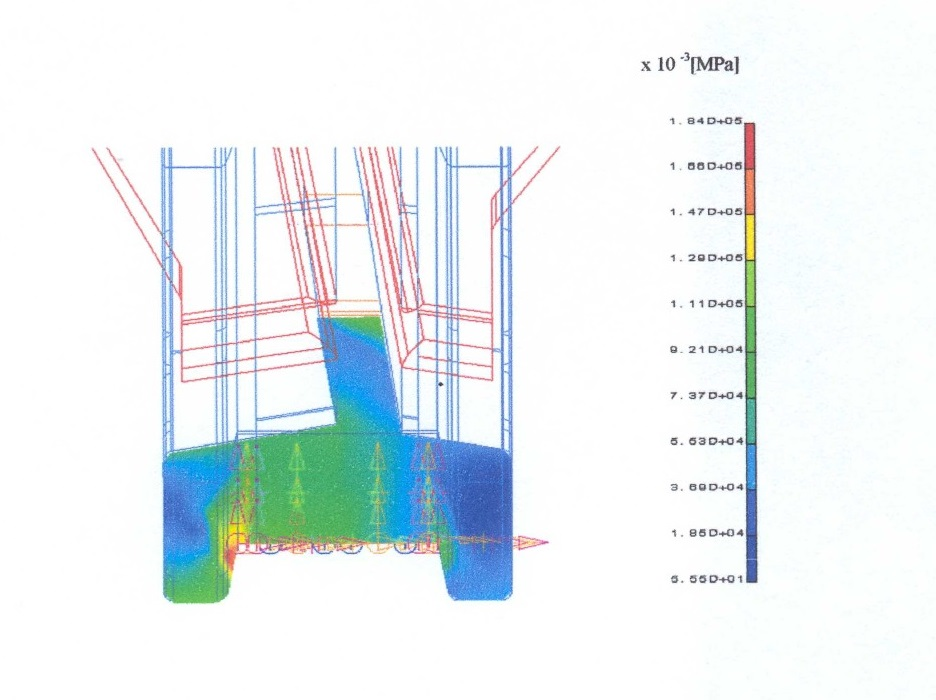
\includegraphics[width=6.85in]{figure/FMANU_MD_04_1274_13.jpg}}
\caption{A figure expanded to double column width the text from Figure~\ref{fig_example3.jpg}}
\label{fig_example4.jpg}
\end{figure*}
%%%%%%%%%%%%%%%% end figure %%%%%%%%%%%%%%%%%%%
An author provided the high resolution image
in Fig.~\ref{fig_example3.jpg}
that was sized to a single column width of 3.25in.  Upon seeing the poor quality of the text, the publisher scaled the image to double column width as shown in Fig.~\ref{fig_example4.jpg}
at which point it took half of a page.  The publisher went on to do this for all eight figures generating four pages of figures that the author did not expect. ASME stopped production of the paper even with the larger figures due to the pixilation of the font.

Clearly the text in this figure is unreadable, and it is doubtful that the author can print the output in a way that it is readable.  This is a problem that the author must solve, not the publisher.

As you might expect, I have many more examples, but in the end the author is the best judge of what is needed in each figure.  ASME simply requires that the image meet a minimum standard for font and line quality, specifically the font should be the appropriate size and not be blurred or pixilated, and that lines should be the appropriate weight and have minimal, preferably no, pixilation or rasterization.


%%%%%%%%%%%%%%%%%%%%%%%%%%%%%%%%%%%%%%%%%%%%%%%%%%%%%%%%%%%%%%%%%%%%%%
\section{Tables}

%%%%%%%%%%%%%%%%%%%%%%%%%%%%%%%%%%%%%%%%%%%%%%%%%%%%%%%%%%%%%%%%%%%%%%
%%%%%%%%%%%%%%%%%%%%%%%%%%%%%%%%%%%%%%%%%%%%%%%%%%%%%%%%%%%%%%%%%%%%%%

All tables should be numbered consecutively  and centered above the table as shown in Table~\ref{table_ASME}. The body of the table should be no smaller than 7 pt.  There should be a minimum two line spaces between tables and text.


%%%%%%%%%%%%%%%%%%%%%%%%%%%%%%%%%%%%%%%%%%%%%%%%%%%%%%%%%%%%%%%%%%%%%%
\section{Citing References}

%%%%%%%%%%%%%%%%%%%%%%%%%%%%%%%%%%%%%%%%%%%%%%%%%%%%%%%%%%%%%%%%%%%%%%
The ASME reference format is defined in the authors kit provided by the ASME.  The format is:

\begin{quotation}
{\em Text Citation}. Within the text, references should be cited in  numerical order according to their order of appearance.  The numbered reference citation should be enclosed in brackets.
\end{quotation}

The references must appear in the paper in the order that they were cited.  In addition, multiple citations (3 or more in the same brackets) must appear as a `` [1-3]''.  A complete definition of the ASME reference format can be found in the  ASME manual \cite{asmemanual}.

The bibliography style required by the ASME is unsorted with entries appearing in the order in which the citations appear. If that were the only specification, the standard {\sc Bib}\TeX\ unsrt bibliography style could be used. Unfortunately, the bibliography style required by the ASME has additional requirements (last name followed by first name, periodical volume in boldface, periodical number inside parentheses, etc.) that are not part of the unsrt style. Therefore, to get ASME bibliography formatting, you must use the \verb+asmems4.bst+ bibliography style file with {\sc Bib}\TeX. This file is not part of the standard BibTeX distribution so you'll need to place the file someplace where LaTeX can find it (one possibility is in the same location as the file being typeset).

With \LaTeX/{\sc Bib}\TeX, \LaTeX\ uses the citation format set by the class file and writes the citation information into the .aux file associated with the \LaTeX\ source. {\sc Bib}\TeX\ reads the .aux file and matches the citations to the entries in the bibliographic data base file specified in the \LaTeX\ source file by the \verb+\bibliography+ command. {\sc Bib}\TeX\ then writes the bibliography in accordance with the rules in the bibliography .bst style file to a .bbl file which \LaTeX\ merges with the source text.  A good description of the use of {\sc Bib}\TeX\ can be found in \cite{latex, goosens} (see how two references are handled?).  The following is an example of how three or more references \cite{latex, asmemanual,  goosens} show up using the \verb+asmems4.bst+ bibliography style file in conjunction with the \verb+asme2ej.cls+ class file. Here are some more \cite{art, blt, ibk, icn, ips, mts, mis, pro, pts, trt, upd} which can be used to describe almost any sort of reference.

%%%%%%%%%%%%%%%%%%%%%%%%%%%%%%%%%%%%%%%%%%%%%%%%%%%%%%%%%%%%%%%%%%%%%%
\section{Conclusions}
The only way to ensure that your figures are presented in the ASME Journal of Mechanical Design in the way you feel is appropriate and meets the requirement for quality presentation is for you to prepare a double column version of the paper in a form similar to that used by the Journal.

This gives you the opportunity to ensure that the figures are sized appropriately, in particular that the labels are readable and match the size of the text in the journal, and that the line weights and resolutions have no pixilation or rasterization.  Poor quality figures are immediately obvious on the printed page, and this detracts from the perceived quality of the journal.

I am pleased to provide advice on how to improve any figure, but this effort must start with a two-column version of the manuscript. Thank you in advance for your patience with this effort, it will ensure quality presentation of your research contributions.



%%%%%%%%%%%%%%%%%%%%%%%%%%%%%%%%%%%%%%%%%%%%%%%%%%%%%%%%%%%%%%%%%%%%%%
\section{Discussions}
This template is not yet ASME journal paper format compliant at this point.
More specifically, the following features are not ASME format compliant.
\begin{enumerate}
\item
The format for the title, author, and abstract in the cover page.
\item
The font for title should be 24 pt Helvetica bold.
\end{enumerate}

\noindent
If you can help to fix these problems, please send us an updated template.
If you know there is any other non-compliant item, please let us know.
We will add it to the above list.
With your help, we shall make this template
compliant to the ASME journal paper format.


%%%%%%%%%%%%%%%%%%%%%%%%%%%%%%%%%%%%%%%%%%%%%%%%%%%%%%%%%%%%%%%%%%%%%%
\begin{acknowledgment}
ASME Technical Publications provided the format specifications for the Journal of Mechanical Design, though they are not easy to reproduce.  It is their commitment to ensuring quality figures in every issue of JMD that motivates this effort to have authors review the presentation of their figures.

Thanks go to D. E. Knuth and L. Lamport for developing the wonderful word processing software packages \TeX\ and \LaTeX. We would like to thank Ken Sprott, Kirk van Katwyk, and Matt Campbell for fixing bugs in the ASME style file \verb+asme2ej.cls+, and Geoff Shiflett for creating
ASME bibliography stype file \verb+asmems4.bst+.
\end{acknowledgment}

%%%%%%%%%%%%%%%%%%%%%%%%%%%%%%%%%%%%%%%%%%%%%%%%%%%%%%%%%%%%%%%%%%%%%%
\begin{nomenclature}
\entry{A}{You may include nomenclature here.}
\entry{$\alpha$}{There are two arguments for each entry of the nomemclature environment, the symbol and the definition.}
\end{nomenclature}

%%%%%%%%%%%%%%%%%

\subsection{Other Thoughts}

The valve can be explained by relatively simple magnetostatics.
In a magnetic field, ferrofluid tends to minimize the potential energy.

Let us first perform a thought experiment.
Consider a two-dimensional magnetic field in the shape of a disc
formed by two sheets of
glass or plastic in, for example,
a circular air gap in a magnetic circuit.
Assume for a moment that the magnetic field is perfectly uniform
within the disc and perfectly zero outside of the disc.
Although there is no gradient in such a scenario, if a connected
blob of ferrofluid enters the disc, it will be pulled entirely
within the disc, since it is magnetically connected to itself
and this minimizes the potential energy, even though there is no
magnetic gradient at any point.
In such a scenario, if the blob is smaller than the disc,
it will not matter where it is inside the blob resides,
since the field is uniform, any is as good as any other.
If however, the blob is larger than the disc, it will tend to
form a circle centered on the disc center.
If the blob is smaller than the disc, it will still self-attract
itself into a circle, but the center of the blob circle might not
coincide with the center of the magnetic disc.

Now let us consider a complex two-dimesional field of arbitrary
shape varying in intensity at every point--for example, it could
be in the shape of a star or a bunny rabbit.
Setting aside for a minute the fact that the ferrofluid will interact
with itself a small amount to vary the shape of this field as it
enters it, we now what the magnetic potential energy at every point
of the boundary of this blob will be the same. If it is not,
it will not be in a minimum energy configuration, and it will
flow until it reaches a minimum configuration. The blob, however or
small, will effectively define an ``isopotential line'' of the
magnetic field.

If we assume the field is radially symmetric, it is clear the
blob will be circular. (Let us ignore a field which had several
local minima energy conditions.)


Now, let use return to a uniform magnetic field of radius
$R$ wish is of strength $B_R$ within this disc and zero
outside it.
Now, what is the potential energy of a ferrfluid blob at
any arbitrary position (before it has sought a minimum)?
For a given patch of ferrfofluid $A$
and the magnetization of the ferrofluid is $M_{A}$
the potential energy is:
\begin{align}
U &= - B_R A M_{A}, \text{if $A$ is with disc $R$,} \\
U &= 0, \text{if $A$ is outside the disc}
\end{align}

Representing this a Kronecker Delta $\delta{A}$,

\[
\delta_{A} =
    \begin{cases}
            1, &         \text{if $A$ is with disc $R$,} \\
            0, &         \text{if $A$ is outside the disc}
    \end{cases}
\]

we can integrate over the entire area, we have:
\[ U = \int_{A} -B_R  M_{A} \delta_{A} \,dA \],
but since $B_R$ does not depend on $A$, we have:
\[ U = -B_R \int_{A}  M_{A} \delta_{A} \,dA \],

If we approximate our magnetic field as ``strong'' within
a small finite boundary and zero elsewhere, and assume that
the within the strong field the ferrofluid reaches its
saturation magnetization $M_s$, we can simplify this further:
\[ U =  -B_R M_{s} \int_{A}   \,dA \]

In other words, the potential energy is minimized by keeping as
much of the ferrorfluid in the disc $R$ as possible.

It is clear from this that if a bubble of air was magically
placed inside the blob of ferrofluid in inside $R$, it would
quickly be pushed out by energy minimization.

But how can we smuggle a bubble of air into the blob?
Well, we can make a thin ``staw'' and pace the end of it inside
the blob. Now, it take no work to displace the blob until
it is pushed outside the disc. Now the ferrofluid will
form the shape of a circle naturally, whether a straw is
pushed into it or not.

If we blow into the straw (in other words, if we raise the
pressure there), the ferrofluid will easily move out of the straw,
making the remainder circular blob bigger---until it starts to
push the ferrofluid outside of the disc. At that point, the
ferrofluid would resist being further displaced.
If, however, there was enough room in the disc for all of the
ferrofluid, even when that inside the valve was displaced,
the air would enter the bolus and then be elimnated to the
other, non-straw boundary of the bolus. In other word, the valve
would have ``cracked'' and allowed the air to pass out.

Now suppose that you push from the other side. The circle would
shrink, and to the extent that the circcle shrinks, that much
ferrofluid would have to be pushed out the straw. However,
if the other end of the straw were at the disc boundary and
a wall prevented the ferrofluid from returning, it would be
removed from the disc. But this requires work, because we are
increasing the energy, by moving away from a minimum energy
configuration.

Unfortunately, we cannot analyze this further without introducing
gradients.
